\documentclass[fontsize=11pt]{article}
\usepackage{amsmath}
\usepackage[utf8]{inputenc}
\usepackage[margin=0.75in]{geometry}
\usepackage{graphicx}

\title{CSC110 Project Proposal: From Sea Level Raising to Global Warming: Analysing the Relationship Between Sea Level and Climate Change}
\author{Jiankun Wei, Ruiting Chen, Yiteng Sun, Weiheng Wang}
\date{Monday, December 14, 2020}

\begin{document}
    \maketitle

    \section*{Problem Description and Research Question}

    Since the industrial revolution, humans have altered the world greatly from polluting the environment to destroying the habitat. We uninhibitedly release greenhouse gases into the air causing global warming, leaving heavy metals around mines to wipe out local plants, deforest Amazon for farming, and gazing. ("Deforestation in Brazilian Amazon surges to 12-year high") As a result, the species extinction rate of the world has soared from one species per decade to six thousand species per year, which has increased sixty thousand-fold! Yet in the past, humans have taken this for granted. We indeed alter the environment and many species go extinct, but it does not affect us. In fact, our metropolis mushroomed all around the world; airplanes flying high above the sky carrying people to explore previously unreachable places; factories had been built across the globe sending manufactured goods to everybody to improve our life. Even the moon, which our ancestors can only fancy about, has been reached. It seems all fine. But does it?\\
    Gradually and unnoticeable by the proud humans, the Earth is altering and a great danger appears on the horizon -- the Raising of the sea level. ("This is what climate change look like") There are two main reasons for raising the sea level, all of them are due to the increasing amount of greenhouse gases in the atmosphere. As there are more and more greenhouse gases released into the air, it begins trapping sunlight which increases the temperature of the Earth. This in turn melts the ice on the north and south pole. The melted water flows into the sea, which raises the sea level. (“Why Are Glaciers and Sea Ice Melting?”) Also, as temperature rises, water tends to expand, directly leading to increased sea levels. Finally, as the sea level increases, more and more ice on the poles will be submerged underwater, and begin to melt itself. This is crucial because as the underlying ice melt, the iceberg fell into the sea which will eventually disappear resulting in a self-enhancing loop. ("NASA Sea Level Change Portal: Thermal Expansion.")\\
    The rising sea level directly affects human society. First, a devastating tsunami will visit the coastline more frequently causing thousands of lives and money. The deconstruction of shelters will also turn people into refugees. What is more, seawater will taint the coastal farms and add salt into the soil which reduces the crop yield. Last but not the least, many cities located near the sea are directly threatened by the rising sea level. Following the current trend, big metropolis like London, San Diego, New York, and countries like the Netherlands will soon be submerged underwater. (Lewis, Sophie)\\

    Given these important threatens, it is emergent to be aware and understand climate change and the rising sea level, and to treat them seriously.\\

    Our research question is \textbf{"How does sea-level change around the world due to climate change?”} 

    \newpage
    \section*{Data-sets Description}
    We gathered sea level data from the University of Hawaii Sea Level center website(UHSLC Legacy Data Portal), and temperature data from datahub. ("Global Temperature Time Series").\\
    More specifically, sea level data is extacted from http://uhslc.soest.hawaii.edu/data/fd.html. The website contains country name, city name, location of the station and some other information, as well as the links to the actural sea level data in different format. We used the sea level data in .csv format extracted from the hourly csv links from this website. Each sea level csv file include the date at which the sea level data collected and the height of sea level in mm. A sample sea level data from one station(Rikitea	France) is shown below. 
    \begin{figure}[h!]
    \centering
    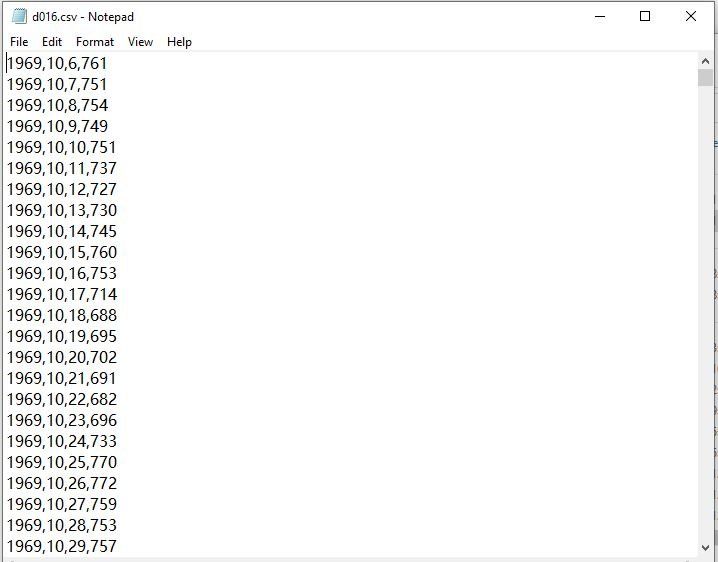
\includegraphics[scale=0.5]{sample_sea_level_data.JPG}
    \caption{Example Sea Level Data}
    \label{fig:sample_sea_level_data.JPG}
    \end{figure}
    The first 3 element of each line represents a date(year, month, day) of the sea level data being collected. The last element of each line is the sea level data in mm. Note that the station name or location is not stored in the csv file, but in the website(picture shown below).
     \begin{figure}[h!]
    \centering
    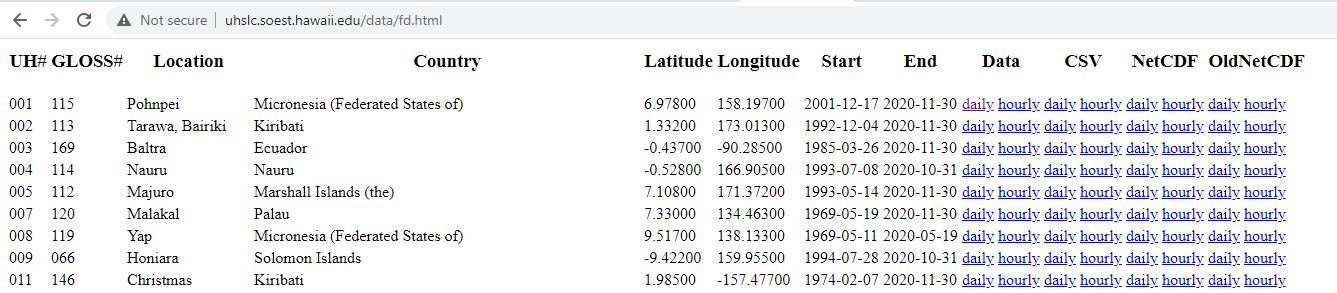
\includegraphics[scale=0.5]{sea_level_website.JPG}
    \caption{Example Sea Level Data Website}
    \label{fig:sea_level_website.JPG}
    \end{figure}
    
    The temperature data is extracted from this link(https://datahub.io/core/global-temp/datapackage.json) to a .jason file provided in this website: https://datahub.io/core/global-temp#python. In the .jason file, we extracted this link(https://pkgstore.datahub.io/core/global-temp/monthly\_csv/data/c1321100952fc1b643ec604ae65a104a/monthly\_csv.csv) to a .csv file of monthly global temperature data. The temperatures in this csv file includes the month of calculated monthly average and two types of temperature data, the Global component of Climate(GCAG) and GISS Surface Temperature (GISTEMP), stored in alternating lines. We used the GCAG data. An example of temperate data is shown below. 
    
    \begin{figure}[h!]
    \centering
    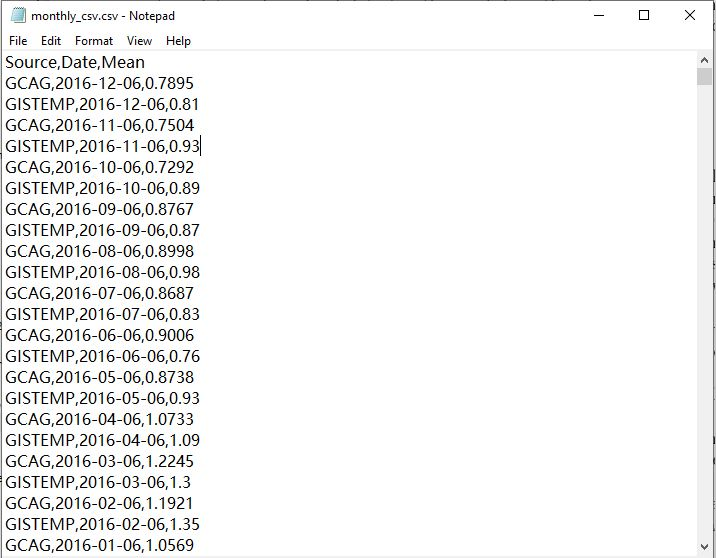
\includegraphics[scale=0.5]{sample_temperature_data.JPG}
    \caption{Example of Temperature Data}
    \label{fig:sample_temperature_data.JPG}
    \end{figure}
    
    \newpage
    The header line in the data set describes the data stored in the data-set. Note that there are 2 types of temperature anomaly data in degree Celsius, GCAG and GISTEMP(2 lines of data), for each month. Here year-month-06 is used to represent the month of temperature data calculated.

    \section*{Computational Plan}

    In order to let the data set be convenient for a computer to use, our group will write functions to read .html format file and .json format file to let python conveniently use this file to do complicated operations and then get assess to the data we need. ("Extracting Data from HTML with BeautifulSoup") Then we will create two dataclasses named "Temperature" and "Station" to recored and store the data we need. In the next step, based on our entities, we would create a new class named "ClimateSeaLevelSystem", which is similar to the system we learnt in the lecture, to store all the data mapping to their key element(like station name matches its corresponding Station). After this step, we could create an abstract class named "EntityGenerator"  and implement two concrete classes inherit from this abstract class to generate the Temperature data and Station separately with its corresponding sea level data and store them in our system "ClimateSeaLevelSystem". Then because the data type in our new data set is the continuous variables in the quantitative data type (Chopra \& Alaudeen(2019) page 1), thus we decide to use linear regression, and the scatter plots on map to present data by using plotly.\\
    We want to present the relationship between the year (x-axis) and average daily sea-level value measured by one station (y-axis). We will first plot all the points out and then draw linear regression based on these points in the graph.\\
    Then, we also design to show the relationship between the year (x-axis) and temperature measured by one station (y-axis). The methods is the same to the steps we take in creating the linear regression of sea level. To find the relation between sea level change and climate change, we will combine two lines in one chart. \\
    Finally, we decided to use plotly to draw a world map with scatter plots about how the sea-level changes at all our stations from around 1980 to 2020, using the sea level data, station data from our data-set. Every single point on the map represents the actual location of each station. In the world map, we decide to use different color of plots to represent whether the sea level of the station is higher or lower than its original height(we also can say the sea level is rising or falling). For stations which reported rising sea level, we will use red to illustrate the sea level raised. For stations that reported falling sea level, we will use blue to illustrate the sea-level falls. Then as time moves forward, the colour will change, given the change in the rising and falling sea level as a vivid animation.\\
    We also change the background ocean colour to reflect the world temperature anomaly. For the time when temperature anomaly is higher that the original measurement, the colour of the ocean will be red. 
    For the time when temperature anomaly is lower that the original measurement, the colour of the ocean will be blue.
    The plotly module has the ability to draw animation which makes it relevant because by using plotly to draw animation, we can have a direct visualization of the data. As we depict the rising and falling of the sea level as time moves forward, the animation conveys in a vivid way the data which is just what we want to study. \\
    Using plotly to draw animation is also appropriate because it reflects how sea level has changed in the recorded time period. This will give us valuable intuition on the data and also the importance of climate change. For example, when you see that as time passes, more and more stations become red, you will immediately realize the significance of climate change on our world and how less time we have. Thus, by viewing the animation, one will realize that the problem of climate change is something that we must treat seriously.

   \section*{Instructions}
   There is no need to download data-sets from anywhere because our program will extract all data-sets needed automatically from the internet. \\
   To run the program, you can just simply run the main.py file,and everything will run automatically. There is no need to explicitly call any functions. Once running, all the instructions that will assist you further exploring our program will be displayed in the python console, and you can just followed it. \\
   More explicitly, when running the main.py file, the program will extract all the temperature and sea level date from the internet and process and add them. After that, an animation will display in your web-browser. 
   

    \begin{figure}[h!]
    \centering
    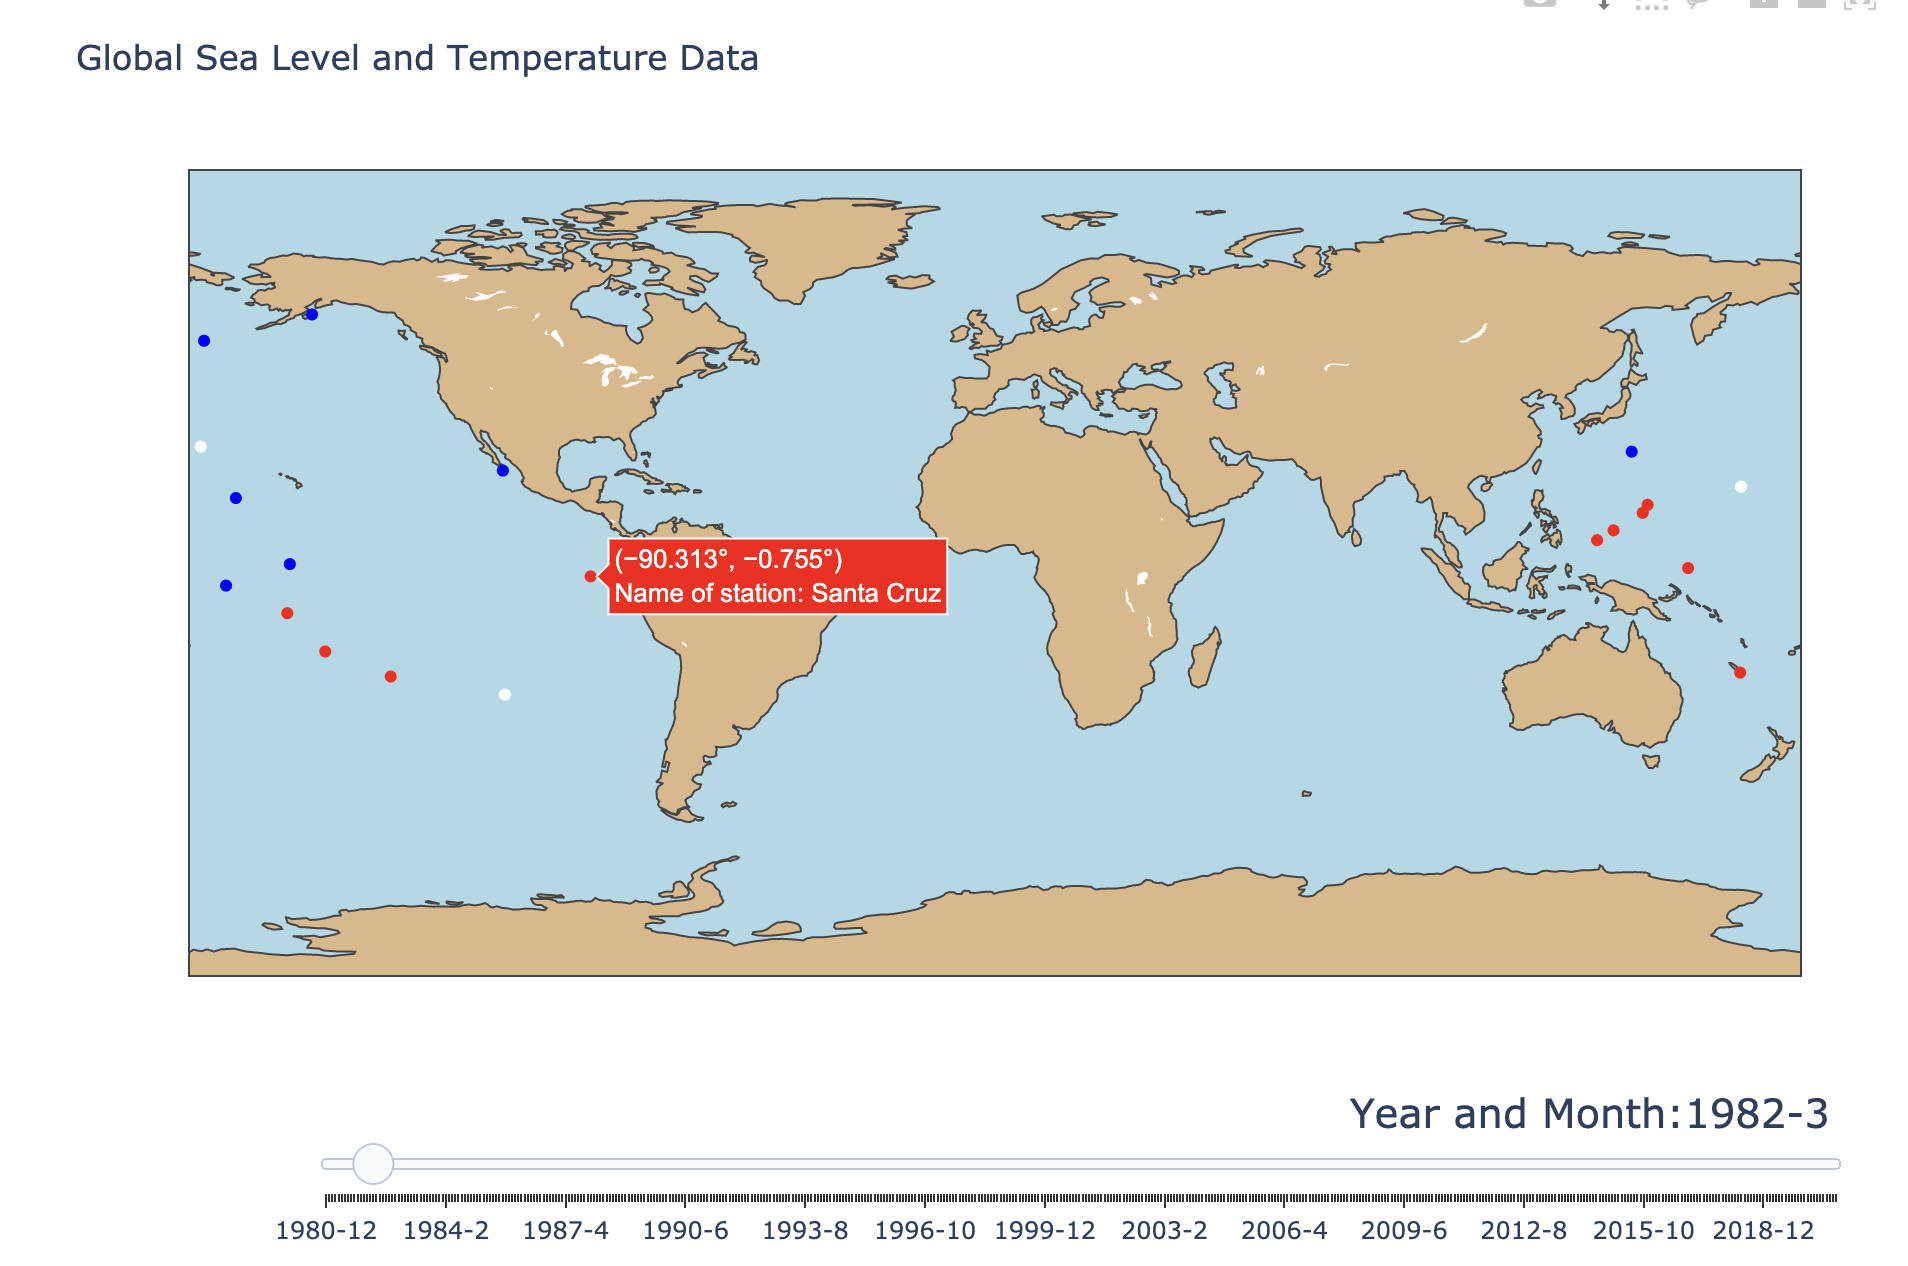
\includegraphics[scale=0.5]{sample_animation_graph.png}
    \caption{Example of Animation Graph}
    \label{fig:sample_animation_graph.png}
    \end{figure}
   
    \section*{}
   As shown in this animation graph, the bottom is a slider with a time line that you can drag to see report of each report of each month of the past many years ( default past 40 years.) At the beginning, the background ocean colour is set to be default light\_blue colour and the colour of each station is set to be blue colour. As time proceed forward, there colours will change. \\
   If the sea level of a station fall below the original sea level of that station, then the colour of that station will be blue. If the sea level of a station raise above the original sea level of that station, then the colour of that station will be red. If there is not sea level measurement of a station during a certain month, the colour of that station will be set to white. 
   Similarly, if the temperature anomaly is less than the original data at the beginning, then the colour of the ocean at that month will be set to blue. On the other hand, if the temperature anomaly is greater than the original data at the beginning, then the colour of the ocean at that month will be set to red. Since the temperature we have is only till 2016, we set the ocean colour of the time after that using the last appeared temperature data.\\
   When you hover over a station, it will show the location and name of that station. You can type the name into python console following the displayed instruction to see the linear regression of all its data as well as the world's temperature anomaly data.\\
   
   \begin{figure}[h!]
   \centering
   \includegraphics[scale=0.35]{sample_station_graph.png}
   \caption{Example of Linear Regression Graph}
   \label{fig:sample_station_graph.png}
   \end{figure}
  
   \section*{}
   As shown in this linear regression graph of the station "Guam", the yellow dots are temperature anomaly data of the world, and the red line is their linear regression.\\
   the green dots are sea level data collected at station "Guam", and the blue line is their linear regression.\\
   If you type in the wrong station name, don't worry. The program will realize that and promote you to type again. You can see data and linear regression of different stations as many times as you like. When you don't want to see any more of them, you can type in "q" to quit.
   
   \section*{Changes}
   \item
   We no longer will draw the histogram because we believe that the linear regression is enough to show convey the main point of this project-- climate change effects sea level around the world.
   
   \item
   We change the data that we use.\\
   First, we add in the temperature data because we previously only have sea level data, and it failed to show the relationship between sea level change around the world and the climate change around the world.\\
   We also change from trying to download the data on our own and write codes to process them to write codes that will extract data directly from the internet. This way, it is convenient not only to us that we don't need to keep track of where we store them on our computer and worrying about them taking too much of computer storage, but also it make the user of our program easier in that them do not need to find and download all the data on their own but can simply click run file in python console, and the program will take care of everything themselves.\\
   
   \item
   Our previous data-sets were stored using .dat file. This time, we use a new data-sets that store data in .csv file which is easy to process.\\
   
   \item
   In order to further explore the relationship between sea level change around the world and the climate change around the world, we decided to, instead of plotting only the sea level data and draw its linear regression, plot the temperature data and sea level data together and draw their linear regression on the same graph. In this way, it is more obvious to people viewing or graph to realize the relationship between climate change and global sea level.\\
   
   \item
   We also changed our plan from using pygame to draw the animation to using plotly after consulting with professor David Liu during an office hour. 
   After that, we decided not to use colour gradient to show the colour but only use blue to represent temperature/sea level drop below the original value and red to represent temperature/sea level raise above the original value.
   
   \item
   Finally, because the data-set we have to work with is to large, and they take very long to process and draw graph, so we can only display the data for pass 40 years to now instead of from pass 50 years to future 50 years.
   
    \section*{Discussion}

    After finishing our programs and running our codes, we get the astonishing results: from December 1980 onwards, as the temperature rising, there were many stations turning "red", which indicated that overall sea level showed a rising trend especially in Atlantic Ocean and North Pacific Ocean. Fortunately, in the recent 13 years, several stations have returned to normal "blue" due to the fact that many countries dedicate to tackle global warning by taking several methods like eliminating the emission of $CO_2$. We also find an interesting fact that at both poles of the earth, as the temperature rising, sea level shows a falling trend, which is an abnormal phenomenon.\\
    However, there are also some drawbacks in our program:\\
    1. The running time of adding the stations to our ClimateSeaLevelSystem depends on the number of stations user wants to generate. The more stations we would like to add, the more time we cost in running this function. Therefore, we set the default number of stations generated to be 20 stations.\\
    2. The data-sets we use misses some sea level data (Maybe because the equipment at the stations malfunctioned or the stations hasn't been built yet at that time), which are replaced by negative numbers. Thus we write codes to delete them. When we run the linear regression function, these points are not included in the graph. As for the animation graph, they are set to be default white colour at the time when measurement is missing so that it will not miss lead viewers.\\
    3. Because of the temperature data-set we used and the sea level data-set we used are different sources, so we do not have temperature measurement at each specific station but an overall temperature anomalies of the whole world. Thus, we use temperature anomaly of the world for each stations. \\
    4. Based on our data-set, we have daily sea level data of each station and monthly temperature data. In order to compare them more intuitively, we have to compute the average sea level in each month. \\
    5. When graphing, we restricted the time limit to pass 40 years because the first world meeting discussing about global warming was held 40 years ago. To recognize this fact and bring people's attention to the significance of global warming, we set the time duration of our animation graph to be 40 years.\\
    6. It is unavoidable that these stations have different established years. Some stations may establish later than our start year (1980). Therefore, different stations has different linear regression graphs.\\
    7. For the integrity of our animation, we filtered out the stations that was built later than 1980.\\
    For our future exploration, we decide to show more details in our world map, like using plotly to draw an animation to show how sea level changes at our stations in selected period (from 1980 to 2020). In our world map, we use different colour(red and blue) to represent the rise or decline of the sea level. In our future assumption, we want to show more direct and intuitive information of sea level changes like using a gradient of colours to show different level of increase and decrease of sea level. For stations which showed the rising sea level, we will use a gradient from yellow to red to illustrate the intensity of how much sea level raised. For stations which showed the falling sea level, we will use a gradient from light blue to dark blue to illustrate the intensity of how much sea-level falls. Then as the time passes by, we can see how the colour of area changes and then get more intuitive details.

    \newpage
    \section*{References}
    \begin{enumerate}
        \item
        Nunez, Christina. “Sea Level Rise, Explained.” Sea Level Rise, Facts and Information, 27 Feb. 2019, www.nationalgeographic.com/environment/global-warming/sea-level-rise/.
        \item
        UHSLC Legacy Data Portal, uhslc.soest.hawaii.edu/data/?fd.
        \item
        Chopra, R., England, A., \& Alaudeen, M. N. (2019). Data science with Python: Combine Python with machine learning principles to discover hidden patterns in raw data. Birmingham: Packt Publishing.
        \item
        “Why Are Glaciers and Sea Ice Melting?” WWF, World Wildlife Fund, www.worldwildlife.org/pages/why-are-glaciers-and-sea-ice-melting.
        \item
        “NASA Sea Level Change Portal: Thermal Expansion.” NASA, NASA, 26 Mar. 2020.\\ sealevel.nasa.gov/understanding-sea-level/global-sea-level/thermal-expansion.
        \item
        Lewis, Sophie. “Rising Sea Levels on Track to Destroy the Homes of 300 Million People by 2050.” CBS News, CBS Interactive, 30 Oct. 2019, www.cbsnews.com/news/rising-sea-levels-on-track-to-destroy-homes-of-300-million-people-by-2050/.
        \item
        Shasta Darlington. "Deforestation in Brazilian Amazon surges to 12-year high". CNN World, CNN. 1 Dec, 2020.\\ https://edition.cnn.com/2020/12/01/americas/deforestation-brazil-amazon-bolsonaro-intl/index.html
        \item
        "This is what climate change looks like". CNN World, CNN. 11 Dec, 2020.\\
        https://edition.cnn.com/2020/12/11/world/gallery/climate-change-effects-penguins-2020-spc/index.html
        \item
        Gaurav Singhal. "Extracting Data from HTML with BeautifulSoup". Pluralsight.\\ https://www.pluralsight.com/guides/extracting-data-html-beautifulsoup
        \item
        "Intro to animations in Python". Graphing Libraries, Plotly. https://plotly.com/python/animations/
        \item
        "Global Temperature Time Series". Datahub, Datahub. https://datahub.io/core/global-temp\#python
        \item
        Hover Text and Formatting. (n.d.). Python | Plotly. https://plotly.com/python/hover-text-and-formatting/
        \item
        Multiple Axes. (n.d.). Python | Plotly. https://plotly.com/python/multiple-axes/
        \item
        World Climate Conference. (2020, August 25). Retrieved December 13, 2020, from\\
        https://en.wikipedia.org/wiki/World\_Climate\_Conference
    \end{enumerate}

% NOTE: LaTeX does have a built-in way of generating references automatically,
% but it's a bit tricky to use so we STRONGLY recommend writing your references
% manually, using a standard academic format like APA or MLA.
% (E.g., https://owl.purdue.edu/owl/research_and_citation/apa_style/apa_formatting_and_style_guide/general_format.html)

\end{document}
